\begin{figure}[ht]
    \centering
    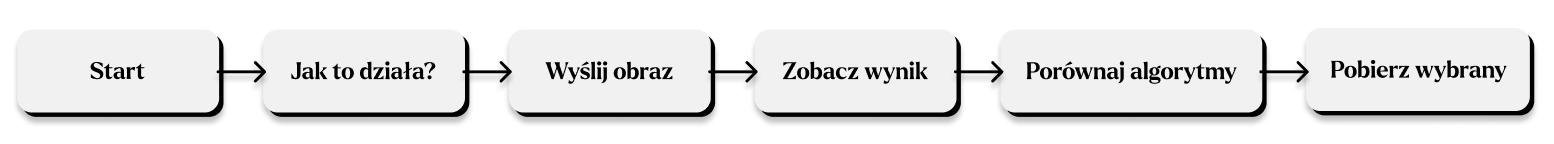
\includegraphics[width=\linewidth]{Rozdziały/06.Aplikacja/Obrazy/user-flow.png}  
    \caption{Diagram przepływu użytkownika}
    \label{fig:image82}
\end{figure}

TODO: Usuń diagram

\section{Implementacja aplikacji}

Po wyborze stosu technologicznego kolejnym krokiem jest skupienie się na implementacji rozwiązań. W tym rozdziale opiszę jakie decyzje podjąłem przy pisaniu kodu aplikacji, jak wygląda struktura aplikacji i jakie problemy napotkałem podczas implementacji.

\subsection*{Struktura aplikacji}

Aplikacja składa się z dwóch części - Frontendu i Backendu. Przy tworzeniu takiego projektu warto zadbać o to, żeby każda część była od siebie niezależna. 

W tym miejscu wracamy do diagramu przepływu użytkownika [Rys \ref{fig:image82}], jak na nim widać, użytkownik nie może wykonać zbyt wiele akcji. Struktura aplikacji jest liniowa, użytkownik 





Schemat blokowy (koncepcyjny) aplikacji

Architektura systemu   

UML

Architektura bazy danych



\begin{table}[ht]
    \centering
    \renewcommand{\arraystretch}{1.5} % Increase row height by 1.25 times
    \begin{tabular}{|l|l|p{8cm}|}
    \hline
    \multicolumn{3}{|c|}{\textbf{Image}}                                                        \\ \hline
    \textbf{Pole}       & \textbf{Typ}          & \textbf{Opis}                                 \\ \hline
    image               & ImageField            & Przesłany obraz.                              \\ \hline
    bilinear\_image     & ImageField            & Obraz powiększony algorytmem Bilinear.        \\ \hline
    dwsr\_image         & ImageField            & Obraz powiększony algorytmem DWSR.            \\ \hline
    esrgan\_image       & ImageField            & Obraz powiększony algorytmem ESRGAN.          \\ \hline
    original\_height    & PositiveIntegerField  & Wysokość oryginalnego obrazu.                 \\ \hline
    original\_width     & PositiveIntegerField  & Szerokość oryginalnego obrazu.                \\ \hline
    dominant\_colors    & TextField             & Pole tekstowe z listą dominujących kolorów.   \\ \hline
    \end{tabular}
    \caption{Struktura bazy danych - Image.}
    \label{tab:image_model}
\end{table}


K-means algorytm do detekcji kolorów wystepujacych na obrazie.


\section{Integracja algorytmów DWSR i ESRGAN}




\section{Testowanie aplikacji}




\section{Wdrożenie i utrzymanie aplikacji}

Omówienie procesu wdrożenia gotowej aplikacji oraz planów dotyczących jej przyszłego utrzymania i aktualizacji.



\section{Plany na przyszłość} \label{sec:plans}

Opis błędów, rzeczy do poprawy w aplikacji. Omówienie jakie są plany rozbudowy aplikacji.

Przyciski nawigacji z widoku do widoku